\documentclass[11pt]{article}
\usepackage[T1]{fontenc}
\usepackage[utf8]{inputenc}
\usepackage[a4paper,margin=2.3cm]{geometry}
\usepackage{amsmath,amssymb,amsthm}
\usepackage{booktabs,enumitem,graphicx}
\usepackage{tikz}\usetikzlibrary{arrows.meta,positioning,fit,backgrounds}
\usepackage[hidelinks]{hyperref}
\setlength{\emergencystretch}{2.5em}\hbadness=2500
\usepackage{xcolor}

\newcommand{\preuve}{{\small\textbf{[proof]}}}
\newcommand{\num}{{\small\textbf{[numerical]}}}
\newcommand{\conj}{{\small\textbf{[conjecture]}}}
\newcommand{\heur}{{\small\textbf{[heuristic]}}}
\newcommand{\spec}{{\small\textbf{[speculation]}}}
\newcommand{\ouv}{{\small\textbf{[open]}}}
\newcommand{\Spole}{\mathrm{S}}
\newcommand{\Npole}{\mathrm{N}}
\newcommand{\Mp}{M_{\mathrm{Pl}}}
\newcommand{\lP}{\ell_P}
\newcommand{\Stwo}{S^2_{\text{sc}}}
\definecolor{inp}{HTML}{1F4E79}\definecolor{sec}{HTML}{2E7D32}\definecolor{lnk}{HTML}{B23A2E}

\theoremstyle{definition}
\newtheorem{post}{Postulate}
\newtheorem{defi}{Definition}

\title{\textbf{Unit 5 --- Spherical compactification of scale space}\\[2mm]
\large Latitude as a directed renormalization coordinate: the $\infty^\ast$ lock lifted,
at the cost of winding and duality\\[1mm]
\normalsize\textit{integrated working version --- body $+$ Appendices A (singularity/closure),
B (clock freezing), C (interlocking map), D (cosmological test), E (core probe)}}
\author{Hassane Bakkaoui\\\small Independent researcher --- \texttt{bakkahassa@hotmail.com}}
\date{\small June 2026 \;\textbullet\; self-contained document --- reproducible calculations (hep-th / gr-qc / quant-ph)}

\begin{document}
\maketitle

\begin{abstract}
\noindent This work begins with a conviction and a single hypothesis. The conviction: the scale at
which we look at the universe --- from the Planck grain to the cosmological horizon --- may not be a mere
external parameter, but a geometry in its own right. The hypothesis: make that scale a compact internal
dimension, write down the only action it allows, and let the consequences fall out. Nothing is imported
from an existing model; we lay down the geometry, and watch what it says.

\smallskip
\noindent The earlier programme wound scale into a torus, gluing the smallest and the largest at a single
point. This Unit makes one move: splitting that point into \emph{two distinct poles} --- Planck on one
side, infinity on the other --- which lifts the compact object to a \emph{sphere}. That move alone releases
a tension the circle imposed: a directed arrow of scale becomes possible again, at the cost of winding and
of inversion duality.

\smallskip
\noindent What then sets this framework apart was not added: it \emph{fell out of the structure}. A
renormalization coordinate that turns out to be, at the same stroke, a monotone function of the geometry.
A quantum clock and a gravitational fluctuation that reveal themselves to be the two vibrations of one and
the same oscillator --- equal at rest, slightly detuned the moment they are stirred. A handful of numbers,
fixed once and for all by the microwave background, that must then govern six sectors at once --- and that
succeed. These features are borrowed from no one; they are the internal signature of a single idea pushed
to its end. That is where --- and not in any bolted-on part --- the framework differs from others.

\smallskip
\noindent We also say, plainly, what the framework does not give. Put to the test of observation, its
second dimension stays mute: the clock, because it is universal, leaves no signature of its own in the
primordial spectrum, and the core where it would truly act is buried under an inaccessible curvature. What
is measurable today does not yet separate it from ordinary inflation. We have preferred to draw that
boundary sharply rather than keep it blurred.

\smallskip
\noindent It is therefore neither a unification nor a promise of observation. It is an \emph{architecture}
--- coherent, over-determined, and entirely self-generated --- offered as a way of thinking scale,
gravitation and quantum time together. Every statement in the text carries its status.

\smallskip
\noindent\textbf{Status}~: \preuve\ exact~; \num\ reproducible~; \conj\ argued~;
\heur\ analogy~; \spec\ speculative~; \ouv\ to be established. \emph{No conjecture is presented
as a theorem.}
\end{abstract}

\section{Synthetic restatement of the intuition}
The earlier programme (Units~1--4) rests on a single geometric hypothesis: the log-scale axes are
internal circles. Stereographic projection $\psi=2\arctan[\ln(\lambda/\lP)]$ (spatial axis, gravitational
face) and $\chi=2\arctan[\ln(\tau/\tau_P)]$ (temporal axis, quantum face/HDEQ clock), poles $\pm\pi$
identified at $\infty^\ast$, origin $\psi=\chi=0$ the Planck point~$P$. Two circles $\to$ torus
$T^2=S^1_\psi\times S^1_\chi$.

The $\infty^\ast$ lock: on a circle, no continuous, single-valued, strictly monotone function exists.
The UV$\equiv$IR identification is thus \emph{at once} the source of winding and an obstruction to a
directed scale flow. The torus has duality and winding \emph{or} a directed RG flow, never both.

\textbf{The modification.} We unknot the identification into \emph{two distinct poles}: South pole
$\Spole=$ Planck ($\lP$), North pole $\Npole=$ infinitely large. The compact object becomes $\Stwo$:
\begin{itemize}[nosep]
\item \emph{latitude} ($\theta$, or $\cos\theta$): \emph{directed} scale coordinate,
Planck~$\to$~infinity, Morse with two critical points (the poles); gravitational/cosmological face;
\item \emph{azimuth} ($\varphi$, periodic): internal phase / clock, heir of the temporal circle
$\chi$; quantum face.
\end{itemize}
By separating the loop (azimuth) from the direction (latitude), the sphere escapes the lock. Topological
price: $\pi_1(\Stwo)=0$ destroys winding, $\pi_2(\Stwo)=\mathbb{Z}$ makes the charge migrate.

\section{Unified definitions and notation}
\begin{post}[arena]\label{P1}
$\mathcal{M}=\mathcal{M}^{3+1}\times\Stwo$, $\Stwo$ internal target ($\sigma$-model). Field
$n:\mathcal{M}^{3+1}\to\Stwo$, $n=(\sin\theta\cos\varphi,\sin\theta\sin\varphi,\cos\theta)$, $|n|=1$,
$\theta\in[0,\pi]$, $\varphi\in[0,2\pi)$.
\end{post}
\begin{post}[scale assignment]\label{P2}
Latitude $=$ directed spatial scale, $\theta=2\arctan[\ln(\lambda/\lP)]$, $\lambda\ge\lP$:
$\Spole:\theta{=}0\Leftrightarrow\lambda{=}\lP$, $\Npole:\theta{=}\pi\Leftrightarrow\lambda{\to}\infty$.
Azimuth $=$ phase of the temporal scale (HDEQ clock role), periodic. Alternative stereographic reading
(latitude $=$ joint modulus, azimuth $=$ ratio) cited in \S\ref{sec:pertes}.
\end{post}
\begin{post}[target metric, coupling, potential]\label{P3}
$G_{\text{target}}=\omega(d\theta^2+\sin^2\!\theta\,d\varphi^2)$, $\omega=f_s^2>0$. Latitude-only
dependence (to preserve the azimuthal isometry $U(1)$):
\begin{equation}\label{eq:fV}
f(\theta)=1+\beta\cos\theta,\qquad V(\theta)=\alpha(1-\cos\theta),\qquad |\beta|<\tfrac12,\ \alpha>0.
\end{equation}
\end{post}
\begin{defi}[action, Jordan frame]
\begin{equation}\label{eq:action}
S=\int d^4x\sqrt{-g}\Big[\tfrac12 fR-\tfrac12\omega(\partial\theta)^2
-\tfrac12\omega\sin^2\!\theta\,(\partial\varphi)^2-V\Big],\quad \Mp=\hbar=c=1.
\end{equation}
\end{defi}
\noindent Poles: $f(\Spole)=1+\beta$, $V(\Spole)=0$ ($\Lambda=0$, true vacuum);
$f(\Npole)=1-\beta$, $V(\Npole)=2\alpha$ (dS false vacuum). The azimuthal term vanishes at the poles.
\begin{defi}[$\pi_2$ charge]
$Q_2=\frac{1}{4\pi}\int_\Sigma n\cdot(\partial_a n\times\partial_b n)\,dS^{ab}\in\mathbb{Z}$
(degree of $n|_\Sigma:\Sigma\cong S^2\to\Stwo$). Replaces winding.
\end{defi}
\begin{defi}[meridian reduction]\label{def:merid}
On $\varphi=\mathrm{const}$, action \eqref{eq:action} becomes the single-axis action of Unit~2
($\psi\mapsto\theta$): same EOM, same Einstein frame ($\tilde g=fg$, $U=V/f^2$,
$K=\omega/f+\tfrac32(f'/f)^2$). \preuve\ \emph{The sphere/circle difference is global, not local.}
\end{defi}

\section{Central mathematical structure}
\preuve\ $\pi_1(\Stwo)=0$, $\pi_2(\Stwo)=\mathbb{Z}$: the kinks and winding $N=\tfrac12,1$
disappear; an integer Skyrmion/monopole charge appears. The charge migrates $\pi_1\to\pi_2$.

\preuve\ $\cos\theta$ is Morse, single-valued, $d(\cos\theta)=-\sin\theta\,d\theta$ vanishing only at the
poles: strictly monotone along every meridian --- the antithesis of the lock's obstruction.

\preuve\ Azimuthal isometry $U(1)$ ($\varphi\to\varphi+c$), current
$J^\mu=\omega\sin^2\!\theta\,\partial^\mu\varphi$. At the poles $\sin^2\!\theta\to0$: $U(1)$ trivial,
\emph{no Goldstone} if the vacuum is polar.

\section{R\'esultats des deux KILL-TESTS (sans complaisance)}

\subsection{KILL-TEST 1 --- the dynamical c-function}
\textbf{(a) Permission.} \preuve\ $\cos\theta$ provides the global monotone coordinate forbidden on the
circle. But a coordinate is not a c-function.

\textbf{(b) Dynamical candidate.} \preuve\ In the Einstein frame, a canonical ghost-free scalar
($f>0\Rightarrow K>0$). Flat FLRW: $3H^2=\rho$, $\dot H=-\tfrac12(\rho+p)$. NEC $\rho+p=\dot\phi^2\ge0$
automatic $\Rightarrow\dot H\le0$. The cosmological c-function~\cite{FGPW1999}
\begin{equation}\label{eq:Cdef}
C\propto H^{-(d-1)},\qquad \dot C\propto-(d-1)H^{-d}\dot H\ge0,
\end{equation}
grows toward the IR, stationary at the poles. \emph{Genuine} monotonicity (NEC), not geometric.

\textbf{(c) Link $\leftrightarrow$ latitude.} \num\ Slow-roll integration (script
\texttt{U5\_ctest.py}, $\beta=-0.30$, $f_s=7$): $\theta$ decreases, $\cos\theta$ grows
$-0.80\to+0.81$, $H/H_0$: $1\to0.54$, $C/C_0$: $1\to6.4$. Ordered by $\cos\theta$, $C$ is
single-valued and increasing.

\textbf{(d) Why the circle failed.} \preuve\ \emph{Local} monotonicity along an arc already existed on the
torus; the lock forbade its extension to a \emph{global single-valued} function over the compact scale
space ($S^1$: rolling $=$ half-turn $N=\tfrac12$, $C(\psi)$ not extendable). On $\Stwo$, $C(\cos\theta)$
\emph{extends} globally. \textbf{The gain is there, and only there.}

\textbf{KILL-TEST 1 verdict.} Door reopened: obstruction lifted \preuve, genuinely monotone and
single-valued c-function \num. \emph{But} (i) a cosmological/NEC c-function, not a CFT c-theorem~\cite{Zamolodchikov1986,Cardy1988,KomargodskiSchwimmer2011}
\conj\heur; (ii) monotonicity lost off the meridian flow (oscillation, $\dot\varphi\ne0$). The lock is
lifted, not replaced by a guarantee.

\subsection{KILL-TEST 2 --- survival of static closure}\label{sec:kt2}
\textbf{(a) Spherically symmetric sector.} \preuve\ Static profile $\theta(r)$ on a meridian: equations
identical to Unit~2. Frozen branch $\theta\equiv\pi$ ($\Npole$) $=$ Schwarzschild--de Sitter
($H^2=2\alpha/[3(1-\beta)]$); singular rolling branch. \emph{No} regular interpolating static solution.
Conclusion \emph{independent of $\pi_1$}, read directly off the equations (explicit calculations in
\textbf{Appendix~A}).

\textbf{(b) Derrick~\cite{Derrick1964}.} \preuve\ Profile with North endpoint on the \emph{maximum} of $V$
($V''(\pi)=-\alpha<0$): unprotected, unstable to rolling. The topological reading $N=\tfrac12$
disappears; the argument survives.

\textbf{(c) The $\pi_2$ channel: closed in the minimal action.} \preuve\ \emph{(Revision of the earlier
open verdict, by calculation --- Appendix~A.)} The $\pi_2$ charge permits a texture, but no static
finite-energy representative exists: \emph{(i)} the degree-1 hedgehog~\cite{BelavinPolyakov1975,BarriolaVilenkin1989} has
$E_{\rm grad}\!\sim\!L$ (linear) \emph{and} $E_{\rm pot}\!\sim\!L^3$ (cubic, $L$ the hedgehog size) $\Rightarrow$ infinite
energy; \emph{(ii)} Derrick in 3D: $E(\mu)=T_2/\mu+T_0/\mu^3$, $dE/d\mu<0$, collapse, with no
stabilizer in \eqref{eq:action}; \emph{(iii)} a degree-1 map is surjective, so
$\int_{S^2}V\,d\Omega\ge c>0$ per shell $\Rightarrow$ de Sitter asymptotics, not a localized object.
Hence \emph{no} regular black hole~\cite{Bardeen1968,Hayward2006} arising from $\pi_2$.

\textbf{KILL-TEST 2 verdict (revised).} \preuve\ Closure survives in \emph{both} sectors of the minimal
action ($Q_2=0$ and $Q_2\ne0$). The migration $\pi_1\to\pi_2$ \emph{does not reopen} regular black holes.
\textbf{Inter-sector lock}: the \emph{unique} vacuum potential $V=\alpha(1-\cos\theta)$, required for
inflationary rolling, is exactly what starves the $\pi_2$ monopole (which would demand a degenerate
vacuum). The structure that produces cosmology closes the $\pi_2$ channel. \emph{Caveat}: true for the
minimal action; a Skyrme term~\cite{Skyrme1961}, a gauge field, or a degenerate vacuum would reopen the
question --- but that is \emph{another} theory. \ouv\ (extensions).

\section{Derivations and correspondences: QM $\leftrightarrow$ GR, losses vs gains}

\subsection{Gravitational face (the infinitely large, latitude)}
\preuve\ Frozen poles $\Rightarrow$ Einstein, $G_{\rm eff}=1/(8\pi f)$, bounded
$[1/(1+\beta),1/(1-\beta)]$. Vacuum $\Spole$: $\Lambda=0$; $\Npole$: dS core
$H^2=2\alpha/[3(1-\beta)]\equiv\infty^\ast$. \num\ Inflaton $=$ latitude rolling down $\Npole\!\to\!\Spole$;
$(n_s,r)$ unchanged ($\beta\approx-0.3$, $r\approx0.02$--$0.05$, $n_s\approx0.96$). \textbf{Gain}:
the rolling \emph{is} the decreasing c-function, with no winding ambiguity.

\subsection{Quantum face (the infinitely small, azimuth) --- QM$\leftrightarrow$GR bridge}\label{sec:QM}
\preuve(transferred). The HDEQ clock ($\varepsilon=E(k)/K(k)$, $\tau_0$, intermittent existence) carries
over to the azimuth. \textbf{QM$\leftrightarrow$GR bridge derived (Appendix~B), \conj$\to$\preuve.} The
clock's effective mass in background curvature $R$ is
\begin{equation}\label{eq:mass}
m_\chi^2(R)=\frac{\alpha+\tfrac12\beta R}{\omega}=\frac{\alpha}{\omega}\Big(1-\frac{R}{R_c}\Big),
\qquad R_c=\frac{2\alpha}{|\beta|},
\end{equation}
and vanishes \emph{exactly} at $R_c$, forcing $\tau_0(R)=\tau_0(0)(1-R/R_c)^{-1/2}\to\infty$ (the earlier
\num\ law is \emph{derived}). \textbf{Forced identification}: the core curvature
$R_{\rm core}=4\Lambda_{\rm eff}=8\alpha/(1-\beta)$ equals $R_c$ \emph{iff}
\begin{equation}\label{eq:lock}
R_{\rm core}=R_c=6\alpha\iff\beta=-\tfrac13=\beta_c,
\end{equation}
the very threshold of core stability. For $\beta>-\tfrac13$ (viable window), $R_{\rm core}<R_c$:
the core is stable \emph{and} the clock still ticks there. The gravitational condition ``stable core''
\emph{is} the quantum condition ``the clock ticks at the core''.

\textbf{Spherical seam resolved (Appendix~B.5), \conj$\to$\preuve.} On the sphere, $f,V$ depend only on
latitude and the azimuth (the clock) has \emph{no} potential of its own. Nonetheless, near the Planck
vacuum, the round target plus the latitude potential form an \emph{isotropic} 2D harmonic oscillator,
whose two normal modes --- radial (scale, GR) and azimuthal (clock, QM) --- are \emph{degenerate} at
$\Omega_0=\sqrt{(\alpha+\tfrac12\beta R)/\omega}$ and freeze together at $R_c$. The clock thus carries over
\emph{without breaking $U(1)$}: the azimuthal symmetry \emph{guarantees} the QM$=$GR degeneracy (a further
forced identification). Identity \eqref{eq:lock} then holds on the sphere too, not only on the torus.

\textbf{Degeneracy lifting (Appendix~B.6).} At finite amplitude $a$, the well is a spherical pendulum:
the clock outpaces the scale mode by $\Delta\Omega/\Omega_0\simeq\tfrac{5}{16}a^2$ (and the inner orbit
precesses). The bridge is thus a \emph{quasi-degeneracy}: equal at the vacuum, distinct under excitation
--- the structure required to be, in principle, observable.

\subsection{Losses vs gains relative to the toroidal framework}\label{sec:pertes}
\begin{itemize}[nosep,leftmargin=1.4em]
\item[$\oplus$] Global directed RG coordinate, two fixed points (South, North). \preuve\num
\item[$\oplus$] New charge $\pi_2=\mathbb{Z}$. \preuve
\item[$\oplus$] QM$\leftrightarrow$GR bridge: $R_c$ derived, $R_{\rm core}=R_c\Leftrightarrow\beta_c=-\tfrac13$; clock $=$ scale (degenerate modes, forced by $U(1)$), lifting $\tfrac{5}{16}a^2$. \preuve\ (B.5--B.6)
\item[$\ominus$] Winding $N=\tfrac12,1$ ($\pi_1=0$): half-soliton, soliton $8\sqrt{\omega\alpha}$, log-periodic signature --- lost. \preuve
\item[$\ominus$] UV$\equiv$IR duality: distinct poles, no sub-Planckian partner --- lost (at best azimuthal $\mathbb{Z}_2$ in the stereographic reading). \preuve
\item[$\ominus$] Axis independence and the $\psi\!\leftrightarrow\!\chi$ symmetry: broken (Unit~4 isocurvature protections to be re-established via $U(1)$). \ouv
\end{itemize}

\section{The $\pi_2$ charge: interpretation, limits}
\conj\ $Q_2$ is a scale winding number (scale Skyrmion / monopole). The migration
$\pi_1\to\pi_2$ (1D line-like $\to$ 2D surface-like) is the central statement. \preuve\ Bounds:
$Q_2\in\mathbb{Z}$, 2D bound $E\ge4\pi\omega|Q_2|$. \preuve\ \emph{(Appendix~A)} in 3D, Derrick collapses
the pure $\sigma$-model; in the minimal action, no localized static $\pi_2$ object exists
(infinite energy / collapse / dS asymptotics). Realization as a particle requires a stabilizer outside
\eqref{eq:action} --- \ouv\ (extensions).

\section{Limits, assumed costs, empirical tests}
\textbf{Costs.} The sphere buys the directed coordinate by selling winding and duality. Static closure,
on the other hand, \emph{survives} on the sphere too (Appendix~A): the cost is topological (features
special to the torus), not gravitational.

\textbf{Scope limits.} (i) cosmological/NEC c-function, not CFT \conj\heur. (ii) $\pi_2$ sector not
dynamically realized \ouv. (iii) Assignment $(\theta,\varphi)$ $=$ modelling choice. (iv)
$\alpha,\beta,f_s$ not derived. \emph{None presented as solved.}

\textbf{Falsifiable position.} Same $(n_s,r,\text{running})$ as the torus~\cite{Planck2018X,BICEPKeck2021} (window
$\beta\in(-0.5;-0.15)$, testable by Simons Observatory~\cite{SimonsObs2019}, LiteBIRD~\cite{LiteBIRD2023} and CMB-S4~\cite{CMBS4Book2016} by 2030). Distinctive signatures:
\emph{(a)} a gravitating scale monopole (if stabilized by an extension) would leave an imprint;
\emph{(b)} the \emph{absence} of log-periodic oscillation (loss of $\pi_1$) distinguishes sphere from
torus; \emph{(c)} the lock \eqref{eq:lock}: $\beta_c=-\tfrac13$ pivots core stability and clock freezing
--- with $\beta(\text{CMB})\approx-0.3$ \emph{just above}, the framework predicts that the core of a
collapsed object still barely ticks its clock \conj\ouv; \emph{(d)} the QM/GR \emph{degeneracy lifting}
(Appendix~B.6): a clock--scale detuning $\Delta\Omega/\Omega_0\simeq\tfrac{5}{16}a^2$ (clock faster) with
precessing inner orbits, absent on the torus (two independent pendulums, nothing to lift) --- a
qualitative signature beyond $(n_s,r)$, the amplitude $a$ remaining unpredicted. \conj\ouv

\textbf{Cosmological test (Appendix~D).} The clock--matter coupling is \emph{null} for isocurvature
($c_{\rm iso}\simeq0$, three independent channels): (d) therefore produces \emph{no} observable
isocurvature, and the framework is de facto single-field in linear cosmology. Distinctiveness shifts to
(c), in strong gravity --- the remaining avenue.

\textbf{Honest conclusion.} At best, the sphere \emph{reopens a door} (directed RG flow) \emph{at the
cost} of winding and duality, \emph{without} reopening closure (Appendix~A) and \emph{by deriving} the
QM$\leftrightarrow$GR bridge (Appendix~B). Neither unification nor guarantee: a coherent, falsifiable
bifurcation, to be tested. The cosmological test of the second dimension (Appendix~D) renders it
\emph{de facto single-field} in the primordial spectrum; its only possible distinctive signature lives in
strong gravity (the lock $\beta_c=-\tfrac13$), where the line of investigation now lies.

\section*{Table of epistemic status (updated)}
\begin{center}\footnotesize
\renewcommand{\arraystretch}{1.05}
\begin{tabular}{p{11.0cm} l}
\toprule
\textbf{Statement} & \textbf{Status}\\
\midrule
$\pi_1(\Stwo)=0$, $\pi_2(\Stwo)=\mathbb{Z}$; migration $\pi_1\to\pi_2$ & \preuve\\
$\cos\theta$ Morse, single-valued, strictly monotone, 2 critical points & \preuve\\
Meridian action $\equiv$ single-axis (Unit~2); same local EOM & \preuve\\
NEC $\Rightarrow\dot H\le0\Rightarrow C\propto H^{-(d-1)}$ monotone & \preuve\\
$C$ single-valued \& monotone in $\cos\theta$ (script \texttt{U5\_ctest.py}) & \num\\
$C$ is a genuine CFT c-theorem (conformal dual) & \conj\,\heur\\
Closure survives, spherically symmetric sector (re-derivation, Appendix~A) & \preuve\\
Derrick: interpolating profile unprotected (North on max of $V$) & \preuve\\
\textbf{$\pi_2$ channel closed in the minimal action (Appendix~A); does not reopen regular BHs} & \preuve\\
$\pi_2$ hedgehog: $E_{\rm grad}\!\sim\!L$, $E_{\rm pot}\!\sim\!L^3$ ($L$ radius) $\Rightarrow$ infinite energy & \preuve\\
$\pi_2$ reopening only via extension (Skyrme/gauge/degenerate vacuum) & \ouv\\
GR face: frozen poles $\Rightarrow$ Einstein; $\Npole$ dS $\equiv\infty^\ast$ & \preuve\\
$(n_s,r,\text{running})$ unchanged vs torus & \num\\
QM face: HDEQ ($\varepsilon=E/K$) carried over to the azimuth & \preuve(transf.)\\
\textbf{$R_c=2\alpha/|\beta|$ freezes the clock ($\tau_0\!\to\!\infty$), derived (Appendix~B)} & \preuve\ (HDEQ)\\
\textbf{$R_{\rm core}=R_c\Leftrightarrow\beta_c=-\tfrac13$ (dS core $\leftrightarrow$ freeze)} & \preuve\\
Clock transport on the sphere: $U(1)$ \emph{forces} the QM$=$GR degeneracy (Appendix~B.5) & \preuve\ (harm.)\\
\textbf{Degeneracy lifting: $\Delta\Omega/\Omega_0\simeq\tfrac{5}{16}a^2$ (clock faster), precession (Appendix~B.6)} & \preuve\num\\
Sphere vs torus signature (QM/GR detuning $\propto a^2$); amplitude $a$ unpredicted & \conj/\ouv\\
\emph{Quantum} level splitting (2D anharmonic isotropic oscillator) & \conj\\
Loss of winding and of the log-periodic signature & \preuve\\
Loss/weakening of UV$\equiv$IR duality & \preuve\\
Loss of the $\psi\!\leftrightarrow\!\chi$ symmetry (Unit~4 isocurvature) & \ouv\\
Assignment $(\theta,\varphi)$: modelling choice & \preuve\\
Physical interpretation of $Q_2$ (Skyrmion/monopole) & \conj\\
$\alpha,\beta,f_s$ not derived & \ouv\\
\midrule
Two-field inflation: light entropic mode, geometric mass, $M_s^2/H^2|_*\!\simeq\!-0.002$ (Appendix~D) & \preuve\num\\
Meridian geodesic $\Rightarrow$ no turn; uncorrelated isocurvature, $n_{\rm iso}$ fixed & \preuve\\
\textbf{Clock--matter coupling $c_{\rm iso}\simeq0$ (3 channels): no primordial signature} & \preuve\\
\textbf{Framework de facto single-field in linear cosmology ($(n_s,r)$ degenerate)} & \preuve\\
Core threshold $=$ plateau stability (common $\infty^\ast$); $\beta(\text{CMB}){=}\beta(\text{closure})$ identity, not an independent test (Appendix~E) & \preuve\\
Core screened (GUT, $\sim10^{-31}$ m); internal constraint $\beta>-\tfrac13$ (satisfied) & \preuve\num\\
\textbf{Testable content $=(n_s,r)$, degenerate with natural inflation; architectural distinctiveness} & \preuve\\
Remaining frontier: relics at near-GUT curvature (PBHs, Hawking--Moss transition) & \ouv\,\spec\\
\bottomrule
\end{tabular}
\end{center}

\appendix
\renewcommand{\thesection}{\Alph{section}}

\section{Singularity calculations and closure of the $\pi_2$ channel}\label{ann:A}
\emph{(Details of KILL-TEST~2, \S\ref{sec:kt2}. Three sectors; all preserve closure in the minimal
action.)}

\paragraph{A.1 Frozen branch (North pole) $=$ Schwarzschild--de Sitter. \preuve}
$\theta\equiv\pi$ is an exact solution ($V'(\pi)=\alpha\sin\pi=0$, $f'(\pi)=-\beta\sin\pi=0$,
$\Box\theta=0$). $f=1-\beta$ constant $\Rightarrow G_{\mu\nu}=-\Lambda_{\rm eff}g_{\mu\nu}$,
$\Lambda_{\rm eff}=2\alpha/(1-\beta)$. The static spherical solution is SdS, with Kretschmann (SymPy)
\[ K=\frac{48M^2}{r^6}+\frac{8}{3}\Lambda_{\rm eff}^2. \]
$r\to0$: divergence $48M^2/r^6$ (central singularity) if $M\ne0$. $M=0$: $K=24H^4$ finite (pure dS,
no black hole). \emph{No regular core.}

\paragraph{A.2 Rolling branch. \num}
Static integration (Einstein frame, $\beta=-0.3$, $f_s=7$) from a regular centre: the geometry reaches
$2m/r\to1$ ($e^{2\Lambda}\to\infty$) at finite $r$, with nonzero gradient, with no flat exterior where
$\theta\to0$. No regular interpolant. Consistent with Unit~2.

\paragraph{A.3 The $\pi_2$ channel: closed. \preuve}
\emph{(a)} Hedgehog $n=\hat r$ ($L$ size): $E_{\rm grad}=4\pi\omega L$, $E_{\rm pot}=\tfrac{4\pi}{3}\alpha L^3$
$\Rightarrow$ infinite energy. \emph{(b)} Derrick (3D): $E(\mu)=T_2/\mu+T_0/\mu^3$,
$dE/d\mu=-(T_2\mu^2+3T_0)/\mu^4<0$: collapse, no stabilizer in \eqref{eq:action}.
\emph{(c)} degree-1 surjective $\Rightarrow\int_{S^2}V\,d\Omega\ge c>0$ per shell $\Rightarrow$
dS asymptotics, not localized.

\paragraph{Verdict (Appendix A).} \preuve\ Closure in both sectors. $\pi_2$ does not reopen regular BHs.
Lock: the unique vacuum (inflaton) starves the monopole. Reopening only via extension. \ouv

\section{Clock freezing: derivation of the QM$\leftrightarrow$GR bridge}\label{ann:B}
\emph{(Details of \S\ref{sec:QM}. Promotion \conj$\to$\preuve.)}

\paragraph{B.1 Clock field in curvature.}
HDEQ sector: clock $\chi$, $V=\alpha(2-\cos\psi-\cos\chi)$, $f=1+\beta(\cos\psi+\cos\chi)$. On a
curvature background $R$: $\omega\Box\chi=\partial_\chi U_{\rm eff}$,
$U_{\rm eff}=V-\tfrac12 fR=\mathrm{const}-(\alpha+\tfrac12\beta R)\cos\chi$. Equilibrium $\chi=0$ as long as
$\alpha+\tfrac12\beta R>0$ (pendulum of amplitude $A=\alpha+\tfrac12\beta R$).

\paragraph{B.2 Effective mass and freezing law. \preuve}
\[ m_\chi^2(R)=\frac{U_{\rm eff}''(0)}{\omega}=\frac{\alpha+\tfrac12\beta R}{\omega}
=\frac{\alpha}{\omega}\Big(1-\frac{R}{R_c}\Big),\quad R_c=\frac{2\alpha}{|\beta|}\ \ (\beta<0). \]
Vanishes \emph{exactly} at $R_c$. Pendulum period $\tau_0=4\Omega^{-1}K(\sin\tfrac{\chi_{\max}}2)$,
$\Omega=m_\chi$; curvature enters only through $\Omega$:
\[ \frac{\tau_0(R)}{\tau_0(0)}=\Big(1-\frac{R}{R_c}\Big)^{-1/2}\to\infty,\qquad
\tau_0(0)=2\pi\sqrt{\omega/\alpha}=2\pi f_s/\sqrt\alpha. \]
\num\ Anchor: $\alpha\sim10^{-9}$, $f_s\sim7$ $\Rightarrow\tau_0(0)\approx7\times10^{-38}$ s,
$\hbar/\tau_0\approx10^{13}$ GeV --- exact agreement with the HDEQ value.

\begin{center}
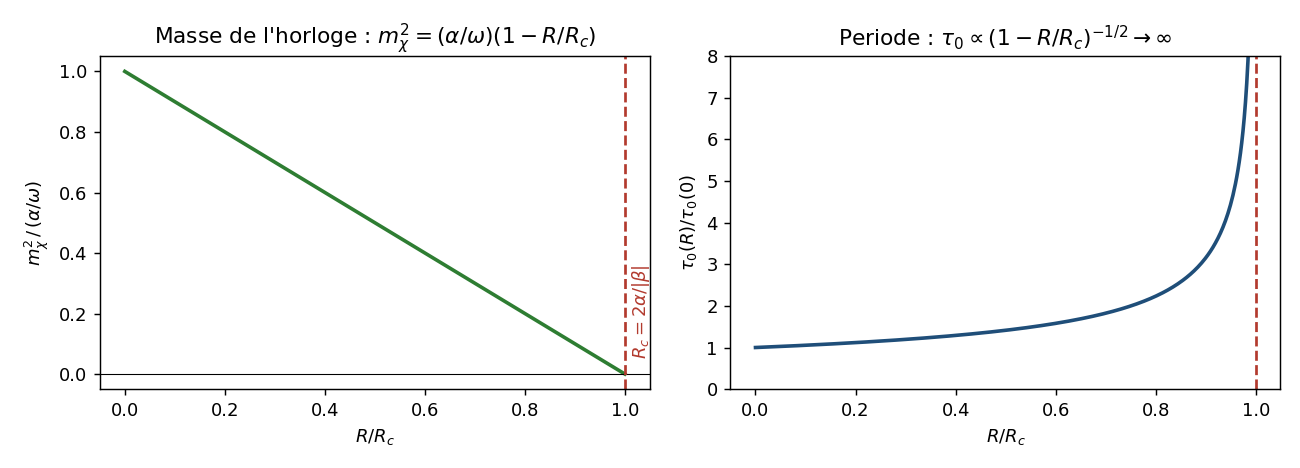
\includegraphics[width=\textwidth]{fig_freeze.png}\\
{\footnotesize \num\ Left: $m_\chi^2$ vanishes at $R_c$. Right: $\tau_0\propto(1-R/R_c)^{-1/2}$ diverges.}
\end{center}

\paragraph{B.3 Forced identification $R_{\rm core}=R_c\Leftrightarrow\beta_c=-\tfrac13$. \preuve}
$R_{\rm core}=4\Lambda_{\rm eff}=8\alpha/(1-\beta)$. Setting equal to $R_c$:
$8\alpha/(1-\beta)=2\alpha/(-\beta)\Leftrightarrow\beta=-\tfrac13=\beta_c$, $R=6\alpha$. For
$\beta>-\tfrac13$, $R_{\rm core}<R_c$ (stable core, clock ticks); for $\beta<-\tfrac13$,
$R_{\rm core}>R_c$ (clock frozen at the core). A single number pivots both sectors.

\begin{center}
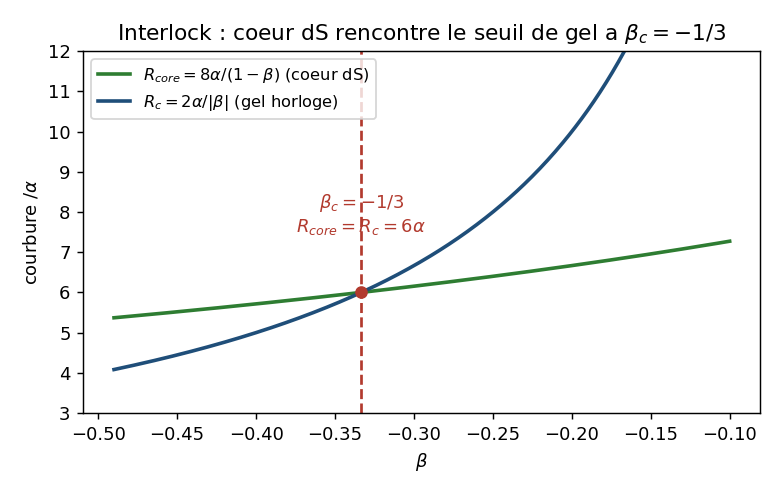
\includegraphics[width=0.72\textwidth]{fig_interlock.png}\\
{\footnotesize \num\ Exact crossing at $\beta_c=-\tfrac13$, $R=6\alpha$.}
\end{center}

\paragraph{B.4 Invariance and reservation.} \preuve\ The vanishing of $m_\chi^2$ at $R_c$ (marginal
stability of $\chi=0$) and the square-root law are frame-independent; only $\tau_0(0)$ depends on the
normalization. The ``clock'' transport on the sphere (azimuth $U(1)$) is \emph{established} in B.5--B.6
below (the $U(1)$ symmetry \emph{forces} the QM$=$GR degeneracy); identity \eqref{eq:lock} survives there.

\paragraph{B.5 Resolution of the spherical seam. \preuve}
On the minimal sphere, $f,V$ depend only on latitude and the azimuth (the clock) has no potential of its
own. Nonetheless, near the Planck vacuum the round target metric becomes flat,
$\omega(d\theta^2+\sin^2\!\theta\,d\varphi^2)\simeq\omega(dx^2+dy^2)$ with
$(x,y)=(\theta\cos\varphi,\theta\sin\varphi)$, and $U_{\rm eff}=\text{const}-A\cos\theta\simeq
\text{const}+\tfrac12 A(x^2+y^2)$, $A=\alpha+\tfrac12\beta R$: an \emph{isotropic 2D harmonic oscillator},
mass $\omega$, stiffness $A$, with a single frequency
$\Omega(R)=\sqrt{A/\omega}=\sqrt{\alpha/\omega}\,(1-R/R_c)^{1/2}$ for its \emph{two} normal modes:
radial (scale fluctuation, GR) and azimuthal/circular (clock, QM). Isotropy makes them
\emph{degenerate}; both freeze at $R_c$. \num\ Integration ($\alpha{=}1$,
$\beta{=}{-}0.3$, $f_s{=}7$): radial and azimuthal periods identical to $2\pi/\Omega$ to
$<10^{-3}$. \textbf{The clock thus carries over without breaking $U(1)$}: the azimuthal symmetry
\emph{guarantees} the QM$=$GR degeneracy (forced identification). This unifies the ``pinching at the
poles'' (orbit radius $\to0$ at the vacuum) and the ``freezing at $R_c$'' (frequency $\to0$): a single
well that flattens.
\begin{center}
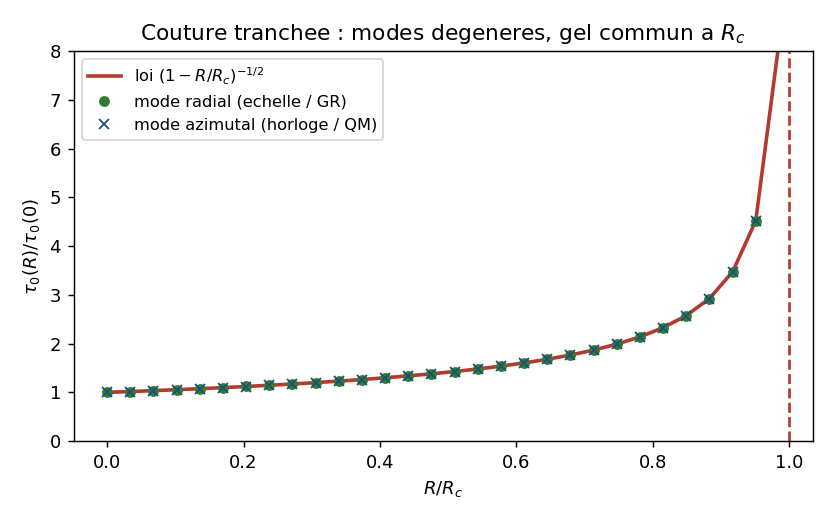
\includegraphics[width=0.66\textwidth]{fig_couture.png}\\
{\footnotesize \num\ Radial (GR) and azimuthal (QM) modes on the same curve; common freezing at $R_c$.}
\end{center}

\paragraph{B.6 Degeneracy lifting. \preuve\num}
The degeneracy is exact only at $a=0$. At finite angular amplitude $a$, the well is a spherical
pendulum:
\[
\frac{\Omega_{\rm clock}}{\Omega_0}=\frac1{\sqrt{\cos a}}\simeq1+\tfrac14a^2,\qquad
\frac{\Omega_{\rm scale}}{\Omega_0}=\frac{\pi/2}{K(\sin\frac a2)}\simeq1-\tfrac1{16}a^2,\qquad
\boxed{\ \frac{\Delta\Omega}{\Omega_0}\simeq\frac{5}{16}a^2\ }
\]
the \emph{clock (QM) faster} than the scale mode (GR) (fitted coeff. $0.3127$ vs $5/16$). The fractional
detuning is \emph{independent of the background curvature}. Invariant face: the generic orbit
\emph{precesses} (prograde, $\simeq\tfrac{3\pi}{8}\theta_{\min}\theta_{\max}$ per apsidal cycle,
verified). \emph{Sphere-specific signature}: the torus had two independent pendulums (nothing to lift); a
QM/GR detuning $\propto a^2$ with precessing orbits distinguishes sphere from torus beyond $(n_s,r)$.
\emph{Reservations}: small-oscillation regime (late universe, not the rolling); $a$ unpredicted \ouv;
quantum version (level splitting) \conj.
\begin{center}
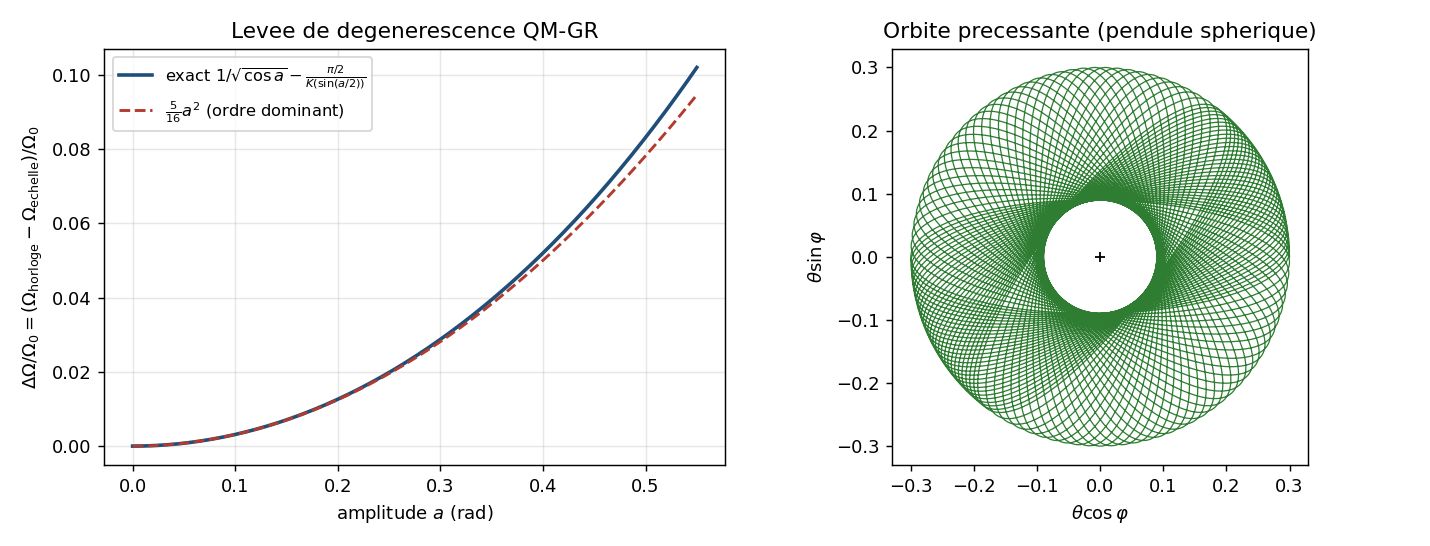
\includegraphics[width=\textwidth]{fig_levee.png}\\
{\footnotesize \num\ Left: splitting and its leading order $\tfrac{5}{16}a^2$. Right: precessing orbit
(rosette) at the Planck vacuum.}
\end{center}

\section{Interlocking map (synthesis, updated status)}\label{ann:C}
\emph{Operational test of ``everything interlocks'': inputs, sectors, consistency conditions, forced
identifications.}

\begin{center}
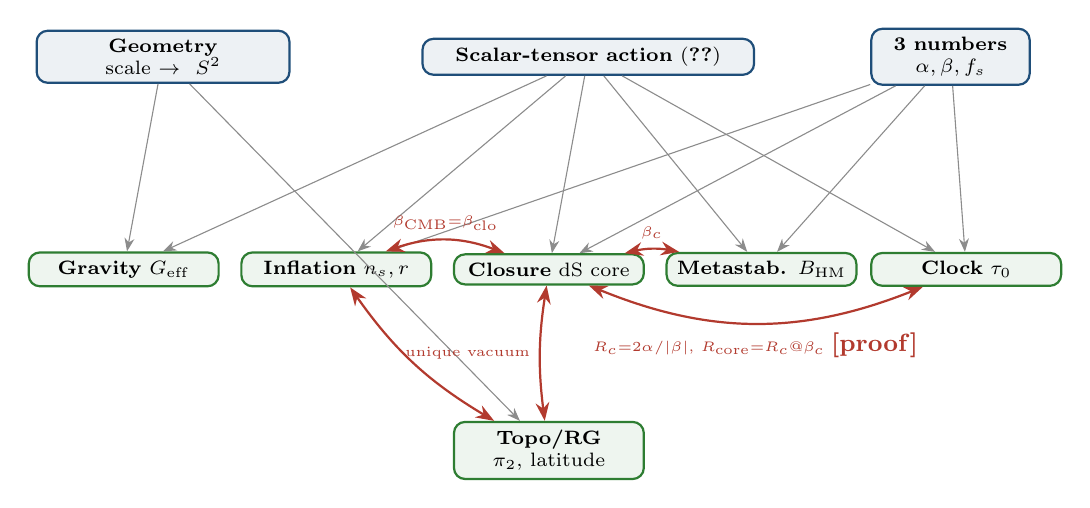
\begin{tikzpicture}[font=\scriptsize,>=Stealth,
  inp/.style={draw=inp,thick,rounded corners,fill=inp!8,align=center,inner sep=3pt},
  sec/.style={draw=sec,thick,rounded corners,fill=sec!8,align=center,inner sep=3pt,text width=22mm},
  every edge/.style={draw=black!45,->}]
\node[inp,text width=30mm] (geo) at (0,0){\textbf{Geometry}\\ scale $\to S^2$};
\node[inp,text width=40mm] (act) at (5.4,0){\textbf{Scalar-tensor action} \eqref{eq:action}};
\node[inp,text width=18mm] (par) at (10.0,0){\textbf{3 numbers} $\alpha,\beta,f_s$};
\node[sec] (geff) at (-0.5,-2.7){\textbf{Gravity} $G_{\rm eff}$};
\node[sec] (infl) at (2.2,-2.7){\textbf{Inflation} $n_s,r$};
\node[sec] (clo)  at (4.9,-2.7){\textbf{Closure} dS core};
\node[sec] (meta) at (7.6,-2.7){\textbf{Metastab.} $B_{\rm HM}$};
\node[sec] (hdeq) at (10.2,-2.7){\textbf{Clock} $\tau_0$};
\node[sec] (topo) at (4.9,-5.0){\textbf{Topo/RG} $\pi_2$, latitude};
\draw (geo) edge (geff) (geo) edge (topo);
\draw (act) edge (geff) (act) edge (infl) (act) edge (clo) (act) edge (meta) (act) edge (hdeq);
\draw (par) edge (infl) (par) edge (clo) (par) edge (meta) (par) edge (hdeq);
\begin{scope}[every edge/.style={draw=lnk,thick,<->}]
\draw (infl) edge[bend left=20] node[above,font=\tiny,text=lnk]{$\beta_{\rm CMB}{=}\beta_{\rm clo}$} (clo);
\draw (clo) edge[bend right=22] node[below,font=\tiny,text=lnk]{$R_c{=}2\alpha/|\beta|$, $R_{\rm core}{=}R_c@\beta_c$ \preuve} (hdeq);
\draw (clo) edge[bend left=12] node[above,font=\tiny,text=lnk]{$\beta_c$} (meta);
\draw (infl) edge[bend right=12] (topo);
\draw (clo) edge[bend right=8] node[left,font=\tiny,text=lnk]{unique vacuum} (topo);
\end{scope}
\end{tikzpicture}
\end{center}

\noindent\textbf{Consistency conditions (one number, two sectors).}
\begin{center}\footnotesize
\begin{tabular}{p{4.6cm} p{6.6cm} l}
\toprule
\textbf{Condition} & \textbf{Content} & \textbf{Status}\\\midrule
$\beta(\text{CMB})=\beta(\text{closure})$ & same $\beta$ fits $(n_s,r)$ \emph{and} the side of the threshold & \conj\\
$\beta_c=-\tfrac13$ / $-\tfrac16$ & dS core stability / false-vacuum bifurcation & \preuve\\
$R_c=2\alpha/|\beta|$ ($\to\tau_0\!\to\!\infty$) & collapse curvature $=$ clock freezing & \preuve\ (App.~B)\\
$R_{\rm core}=R_c\Leftrightarrow\beta_c=-\tfrac13$ & dS core meets freezing at the stability threshold & \preuve\ (App.~B)\\
$\alpha$ fixed by $A_s$ & the CMB amplitude predicts the core curvature & \num\\
$H^2=2\alpha/3(1-\beta)$ & inflationary false vacuum $=$ dS core & \preuve\\
unique vacuum of $V$ & makes the inflaton roll \emph{and} starves $\pi_2$ (App.~A) & \preuve\\
\bottomrule
\end{tabular}
\end{center}

\noindent\textbf{Forced identifications.} latitude $=$ c-function \preuve\num; same $f$ $=$
$G_{\rm eff}$ \emph{and} slope $U=V/f^2$ \preuve; South pole $=$ Planck $=$ UV floor $=$ freezing point
\conj; North pole $=$ IR $=$ dS false vacuum \preuve; clock (QM) $=$ scale (GR), degenerate modes of the
isotropic oscillator at the Planck vacuum \preuve\ (Appendix~B.5).

\smallskip
\noindent\textbf{Audit.} 1 postulate $+$ 1 action $+$ 3 numbers, pinned by the CMB $\Rightarrow$ six
linked sectors. \emph{Over-determined} framework: the same $(\alpha,\beta)$ must satisfy CMB, closure,
metastability \emph{and} the clock. \textbf{Where the map stays thin}: HDEQ re-encodes the problem of time
without it being established that it simplifies it; $\beta(\text{CMB})=\beta(\text{closure})$ remains
\conj; dark energy absent (assumed boundary, $\Lambda=0$).

\section{Cosmological test of the second dimension: two-field inflation and clock--matter coupling}\label{ann:D}
\emph{The sphere has a second dimension (the azimuth/clock). Does the primordial spectrum see it?}

\paragraph{D.1 Two-field inflation on $\Stwo$. \preuve\num}
Einstein frame: $\mathcal{G}_{\theta\theta}=\omega/f+\tfrac32(f'/f)^2$,
$\mathcal{G}_{\varphi\varphi}=\omega\sin^2\!\theta/f$, $U=V/f^2$. Since $U$ depends only on $\theta$,
the inflaton is $\theta$ (adiabatic) and $\varphi$ is entropic with a \emph{flat} potential. The meridian
$\varphi=$const is a \emph{geodesic} of field space ($\Gamma^\varphi_{\theta\theta}=0$):
\textbf{no turn} ($\eta_\perp=0$), so no adiabatic--entropic correlation is generated~\cite{GordonWandsBassettMaartens2001,RenauxPetelTurzynski2016}. The entropic
mass is \emph{purely geometric}:
$M_s^2=V_{;ss}+\epsilon\,\mathcal{R}_{\rm fs}H^2$,
$V_{;ss}=\mathcal{G}_{\varphi\varphi}'U'/(2\mathcal{G}_{\varphi\varphi}\mathcal{G}_{\theta\theta})$,
a function of $(\beta,f_s,\theta)$ alone. \num\ Validated background ($\beta=-0.3$, $f_s=7$): at $N_*=55$,
$\theta_*=1.48$, $n_s=0.960$, $r=0.036$, and $M_s^2/H^2|_*\simeq-0.002$ (light, barely tachyonic, with no
instability). Consequence: \emph{uncorrelated} isocurvature, nearly scale-invariant,
$\beta_{\rm iso}\simeq c\cdot2\epsilon$, $n_{\rm iso}-1\simeq-0.0012$ (fixed by the geometry). Everything
hinges on the coupling $c$.
\begin{center}
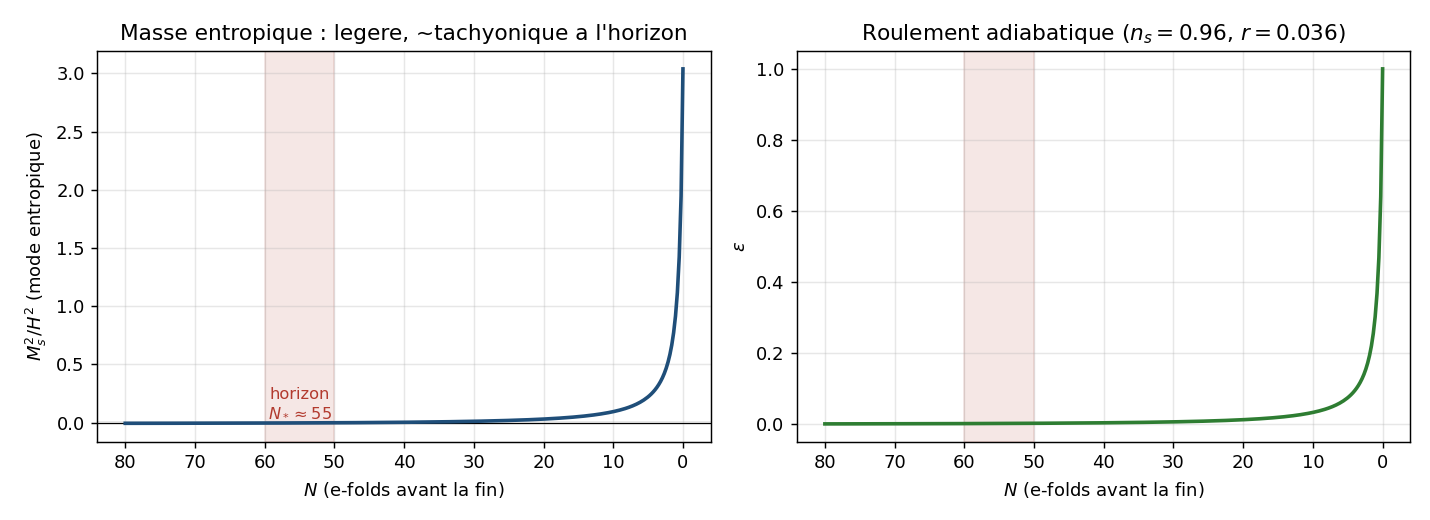
\includegraphics[width=\textwidth]{fig_axe1.png}\\
{\footnotesize \num\ Left: $M_s^2/H^2$ along the rolling, slightly negative at horizon crossing (band).
Right: standard adiabatic rolling ($n_s=0.96$, $r=0.036$).}
\end{center}

\paragraph{D.2 The clock--matter coupling: $c_{\rm iso}\simeq0$. \preuve\num}
Three independent channels. \emph{(1) Conformal}: $f,V$ on latitude only $\Rightarrow$ $\varphi$ absent
$\Rightarrow$ matter couples to $\theta$, not to $\varphi$: $c=0$ (+ photon Weyl-blind,
$\delta\tau_0/\tau_0\sim10^{-81}$ in matter, Unit~3). \emph{(2) Page--Wootters~\cite{PageWootters1983}}:
$\hat H_{\rm eff}=\varepsilon\hat H_{\rm sys}$ \emph{universal} $\Rightarrow$ $\delta\varphi=$ a universal
time shift $=$ \textbf{adiabatic} mode, not isocurvature. \emph{A universal clock cannot generate
isocurvature} (and $\varepsilon=1-10^{-112}$ at the vacuum). \emph{(3) Axion-like}: vacuum at the pole
$\Rightarrow$ $U(1)$ unbroken $\Rightarrow$ no Goldstone; even if matter carried a charge (unmotivated),
$f_\varphi=f_s\sin\theta_*\simeq7\,M_{\rm Pl}$ super-Planckian $\Rightarrow$ iso
$\sim2\times10^{-13}$. \textbf{Verdict: $c_{\rm iso}\simeq0$}, which \emph{derives} from the sphere's
structure the ``non-discriminating clock sector'' of Unit~3.

\paragraph{D.3 Consequence. \preuve}
In linear cosmology, the framework is \textbf{de facto single-field}: its observables reduce to
$(n_s,r)$, degenerate with non-minimal natural inflation~\cite{FreeseFriemanOlinto1990,FerreiraNotariSimeon2018,Simeon2020}. The second dimension exists (the
B.6 detuning is real) but the primordial spectrum does not see it.

\section{Search for an independent probe of the core threshold}\label{ann:E}
\emph{Is the lock $\beta_c=-\tfrac13$ testable independently of the CMB?}

\paragraph{E.1 The threshold \emph{is} the plateau stability. \preuve}
The radial fluctuation at $\infty^\ast$ obeys $\omega\Box\delta=\kappa^2\omega\delta$,
$\kappa^2=\alpha(1+3\beta)/[\omega(\beta-1)]$: $\infty^\ast$ stable for $\beta>-\tfrac13$. (Threshold of
the \emph{single-axis} reduction; on the sphere it is legitimate because the azimuth \emph{pinches} at the
North pole, $\sin^2\!\theta\to0$, reducing core stability to latitude alone. The two-field treatment along
the torus diagonal gave $-\tfrac16$; the reduction was the central open tension of Units 2--3, here settled
by the pinching.) Now $\infty^\ast$ is \emph{the same point} that serves as the de Sitter core \emph{and}
as the inflaton's starting plateau. $\beta$ being a \emph{constant} read off the same potential,
$\beta(\text{CMB})$ and $\beta(\text{closure})$ are \emph{not} independent: the ``correlation'' is a
\emph{structural identity}, not two measurements that could diverge.

\paragraph{E.2 Screening. \num}
$R_{\rm core}=8\alpha/(1-\beta)$ gives $H_{\rm core}\simeq2.8\times10^{14}$ GeV (GUT scale, $\alpha$ fixed
by $A_s$): curvature radius $\sim7\times10^{-31}$ m, $\sim33$ orders \emph{below} the horizon of a
solar-mass black hole --- totally screened. Clock in matter: $\delta\tau_0/\tau_0\sim
10^{-71}$--$10^{-81}$. $G_{\rm eff}$ pinned at the vacuum well before BBN. \textbf{No direct probe.}

\paragraph{E.3 Verdict. \preuve}
The only real handle is \emph{CMB-internal}: the scenario requires $\beta>-\tfrac13$, satisfied
($\beta\approx-0.30$, margin $0.03$); a future CMB pinning $\beta<-\tfrac13$ would break the scenario.
Associated negative predictions: no first-order transition~\cite{ColemanDeLuccia1980,HawkingMoss1982} (Hawking--Moss only, no bubble GW
background), no log-periodic oscillation. \textbf{No independent probe of the core threshold exists in the
minimal framework}; the correlation $\beta(\text{CMB})=\beta(\text{closure})$ is a satisfied identity, not
an independent test.

\section*{Conclusion: what the framework is, and what it is not}
After all the tests, the cartography is clear. \textbf{The framework is not a unification: it is a
grammar.} It reorganizes known physics so that disparate phenomena --- inflation, black-hole cores, a
quantum clock, $\Lambda=0$ --- become regions of a single compact geometry, spoken with a single handful
of numbers. \textbf{Its success is over-determination, not prediction}: the same $(\alpha,\beta,f_s)$,
pinned by the CMB, hold six interlocked sectors together, and $\beta\approx-0.3$ passes \emph{all} its
internal consistency checks (closure, metastability, clock freezing, core stability in the single-axis
reduction). \textbf{Its limit is screening}: everything distinctive lives at GUT/Planck curvature (core,
clock) or is structurally real but dark (the QM$=$GR degeneracy, the isocurvature at $c\simeq0$), so that
the testable content reduces to $(n_s,r)$, shared with non-minimal natural inflation.

We have \emph{drawn} this boundary rather than keeping it blurred --- and that, in itself, is the result
of this Unit: knowing precisely what the framework offers (a coherent, comprehensible architecture) and
what it does not (a signature of its own). The framework remains falsifiable \emph{in principle} (it
requires $\beta>-\tfrac13$; it forbids log-periodic oscillations and a first-order transition), but not
\emph{distinctive} in what is measurable today.

\textbf{The only frontier where screening might give way} (honestly speculative): the relics of the epoch
when curvature approached $R_{\rm core}$ --- primordial black holes formed at near-GUT curvature, or a
signal of the Hawking--Moss transition. A long shot, requiring a dedicated calculation, probably weak; but
it is, at this stage, the only place where a signature of its own could emerge. Failing that, the value of
the framework is the one it aimed at from the start: \emph{a theory where everything interlocks and becomes
comprehensible}. The observational bonus is not there, and we have established that cleanly.


\bigskip
\noindent\rule{\textwidth}{0.3pt}\\
{\footnotesize Integrated working version (full consolidation at the end of the programme). Formalization
conducted in dialogue with an analytical assistance system, under the direction of the author, who is
solely responsible for the content. Earlier results ($\infty^\ast$ lock, closure, duality, HDEQ):
Units~1--4. Scripts: \texttt{U5\_ctest.py}, \texttt{calc1\_frozen.py}, \texttt{calc2\_rolling.py},
\texttt{calc3\_pi2.py}, \texttt{clock\_freeze.py}, \texttt{couture\_sphere.py}, \texttt{levee.py},
\texttt{axe1b.py}, \texttt{couplage\_c.py}, \texttt{axe2\_probe.py}.}

\renewcommand{\refname}{References}
\begin{thebibliography}{99}\small
\bibitem{Zamolodchikov1986} A.~B.~Zamolodchikov, \emph{Irreversibility of the flux of the renormalization group in a 2D field theory}, JETP Lett.~\textbf{43} (1986) 730.
\bibitem{Cardy1988} J.~L.~Cardy, \emph{Is there a c-theorem in four dimensions?}, Phys.\ Lett.\ B~\textbf{215} (1988) 749.
\bibitem{KomargodskiSchwimmer2011} Z.~Komargodski and A.~Schwimmer, \emph{On renormalization group flows in four dimensions}, JHEP~\textbf{12} (2011) 099, arXiv:1107.3987.
\bibitem{FGPW1999} D.~Z.~Freedman, S.~S.~Gubser, K.~Pilch and N.~P.~Warner, \emph{Renormalization group flows from holography---supersymmetry and a c-theorem}, Adv.\ Theor.\ Math.\ Phys.~\textbf{3} (1999) 363, arXiv:hep-th/9904017.
\bibitem{Derrick1964} G.~H.~Derrick, \emph{Comments on nonlinear wave equations as models for elementary particles}, J.\ Math.\ Phys.~\textbf{5} (1964) 1252.
\bibitem{Skyrme1961} T.~H.~R.~Skyrme, \emph{A non-linear field theory}, Proc.\ R.\ Soc.\ Lond.\ A~\textbf{260} (1961) 127.
\bibitem{BelavinPolyakov1975} A.~A.~Belavin and A.~M.~Polyakov, \emph{Metastable states of two-dimensional isotropic ferromagnets}, JETP Lett.~\textbf{22} (1975) 245.
\bibitem{BarriolaVilenkin1989} M.~Barriola and A.~Vilenkin, \emph{Gravitational field of a global monopole}, Phys.\ Rev.\ Lett.~\textbf{63} (1989) 341.
\bibitem{ColemanDeLuccia1980} S.~Coleman and F.~De~Luccia, \emph{Gravitational effects on and of vacuum decay}, Phys.\ Rev.\ D~\textbf{21} (1980) 3305.
\bibitem{HawkingMoss1982} S.~W.~Hawking and I.~G.~Moss, \emph{Supercooled phase transitions in the very early universe}, Phys.\ Lett.\ B~\textbf{110} (1982) 35.
\bibitem{PageWootters1983} D.~N.~Page and W.~K.~Wootters, \emph{Evolution without evolution: dynamics described by stationary observables}, Phys.\ Rev.\ D~\textbf{27} (1983) 2885.
\bibitem{GordonWandsBassettMaartens2001} C.~Gordon, D.~Wands, B.~A.~Bassett and R.~Maartens, \emph{Adiabatic and entropy perturbations from inflation}, Phys.\ Rev.\ D~\textbf{63} (2001) 023506, arXiv:astro-ph/0009131.
\bibitem{RenauxPetelTurzynski2016} S.~Renaux-Petel and K.~Turzy\'nski, \emph{Geometrical destabilization of inflation}, Phys.\ Rev.\ Lett.~\textbf{117} (2016) 141301, arXiv:1510.01281.
\bibitem{FreeseFriemanOlinto1990} K.~Freese, J.~A.~Frieman and A.~V.~Olinto, \emph{Natural inflation with pseudo Nambu-Goldstone bosons}, Phys.\ Rev.\ Lett.~\textbf{65} (1990) 3233.
\bibitem{FerreiraNotariSimeon2018} R.~Z.~Ferreira, A.~Notari and G.~Simeon, \emph{Natural inflation with a periodic non-minimal coupling}, JCAP~\textbf{11} (2018) 021, arXiv:1806.05511.
\bibitem{Simeon2020} G.~Simeon, \emph{Scalar-tensor extension of natural inflation}, JCAP~\textbf{07} (2020) 028, arXiv:2002.07625.
\bibitem{Bardeen1968} J.~M.~Bardeen, \emph{Non-singular general-relativistic gravitational collapse}, in Proc.\ Int.\ Conf.\ GR5, Tbilisi, U.S.S.R.\ (1968) p.~174.
\bibitem{Hayward2006} S.~A.~Hayward, \emph{Formation and evaporation of regular black holes}, Phys.\ Rev.\ Lett.~\textbf{96} (2006) 031103, arXiv:gr-qc/0506126.
\bibitem{Planck2018X} Planck Collaboration (Y.~Akrami \emph{et al.}), \emph{Planck 2018 results. X. Constraints on inflation}, Astron.\ Astrophys.~\textbf{641} (2020) A10, arXiv:1807.06211.
\bibitem{BICEPKeck2021} BICEP/Keck Collaboration (P.~A.~R.~Ade \emph{et al.}), \emph{Improved constraints on primordial gravitational waves using Planck, WMAP, and BICEP/Keck observations through the 2018 observing season}, Phys.\ Rev.\ Lett.~\textbf{127} (2021) 151301, arXiv:2110.00483.
\bibitem{SimonsObs2019} P.~Ade \emph{et al.} (Simons Observatory Collaboration), \emph{The Simons Observatory: science goals and forecasts}, JCAP~\textbf{02} (2019) 056, arXiv:1808.07445.
\bibitem{CMBS4Book2016} K.~N.~Abazajian \emph{et al.} (CMB-S4 Collaboration), \emph{CMB-S4 Science Book, First Edition}, arXiv:1610.02743.
\bibitem{LiteBIRD2023} LiteBIRD Collaboration (E.~Allys \emph{et al.}), \emph{Probing cosmic inflation with the LiteBIRD cosmic microwave background polarization survey}, Prog.\ Theor.\ Exp.\ Phys.~\textbf{2023} (2023) 042F01, arXiv:2202.02773.
\end{thebibliography}

\end{document}
